\let\negmedspace\undefined
\let\negthickspace\undefined
\documentclass[journal]{IEEEtran}
\usepackage[a5paper, margin=10mm, onecolumn]{geometry}
%\usepackage{lmodern} % Ensure lmodern is loaded for pdflatex
\usepackage{tfrupee} % Include tfrupee package

\setlength{\headheight}{1cm} % Set the height of the header box
\setlength{\headsep}{0mm}     % Set the distance between the header box and the top of the text

\usepackage{gvv-book}
\usepackage{gvv}
\usepackage{cite}
\usepackage{amsmath,amssymb,amsfonts,amsthm}
\usepackage{algorithmic}
\usepackage{graphicx}
\usepackage{textcomp}
\usepackage{xcolor}
\usepackage{txfonts}
\usepackage{listings}
\usepackage{enumitem}
\usepackage{mathtools}
\usepackage{gensymb}
\usepackage{comment}
\usepackage[breaklinks=true]{hyperref}
\usepackage{tkz-euclide} 
\usepackage{listings}
% \usepackage{gvv}                                        
\def\inputGnumericTable{}                                 
\usepackage[latin1]{inputenc}                                
\usepackage{color}                                            
\usepackage{array}                                            
\usepackage{longtable}                                       
\usepackage{calc}                                             
\usepackage{multirow}                                         
\usepackage{hhline}                                           
\usepackage{ifthen}                                           
\usepackage{lscape}
\usepackage{circuitikz}


\author{EE25BTECH11041-Naman Kumar }
\graphicspath{./figs/}

\begin{document}
\begin{center}
    \huge{1.9.29}\\
    \large{EE25BTECH11041 - Naman Kumar}
\end{center}
Question:\\
Find the value of y for which the distance between the points $\Vec{A}\brak{3,-1}$ and $\Vec{B}\brak{11,y}$ is 10 units.\\
\solution \\
Distace Between any two vectors = 
\begin{align}
D= \lVert \vec{A}-\vec{B}\rVert
\end{align}
Where
\begin{equation}
\lVert \vec{A}-\vec{B}\rVert=\sqrt{(\vec{A}-\vec{B})^{T}(\vec{A}-\vec{B})} \label{2}
\end{equation}
Given,
\begin{align}
    \vec{A}=\begin{myvec}{3\\-1} \end{myvec}
    \vec{B}=\begin{myvec}{11\\y} \end{myvec}
\end{align}
and distance, D = 10\\
Now using values of Both \textbf{A} and \textbf{B},
\begin{align}
    \vec{A}-\vec{B}=\begin{myvec}{3-11\\-1-y} \end{myvec}
\end{align}
Next
\begin{align}
    (\vec{A}-\vec{B})^{T}(\vec{A}-\vec{B}) = \begin{myvec}{3-11&-1-y} \end{myvec} \begin{myvec}{3-11\\-1-y} \end{myvec}
\end{align}
Putting values in $\eqref{2}$
\begin{align}
    \sqrt{(3-11)^2+(-1-y)^2}=10\\
    (3-11)^2+(-1-y)^2=100\\
    64+1+y^2+2y=100\\
    y^2+2y-35=0\\
    (y+7)(y-5)=0\\
    y=-7 \text{ or } 5 
\end{align}
Therefore, there are two possible values of $\Vec{B}\brak{11,5}$ or $\Vec{B}\brak{11,-7}$
\newpage
\begin{figure}[H]
    \centering
    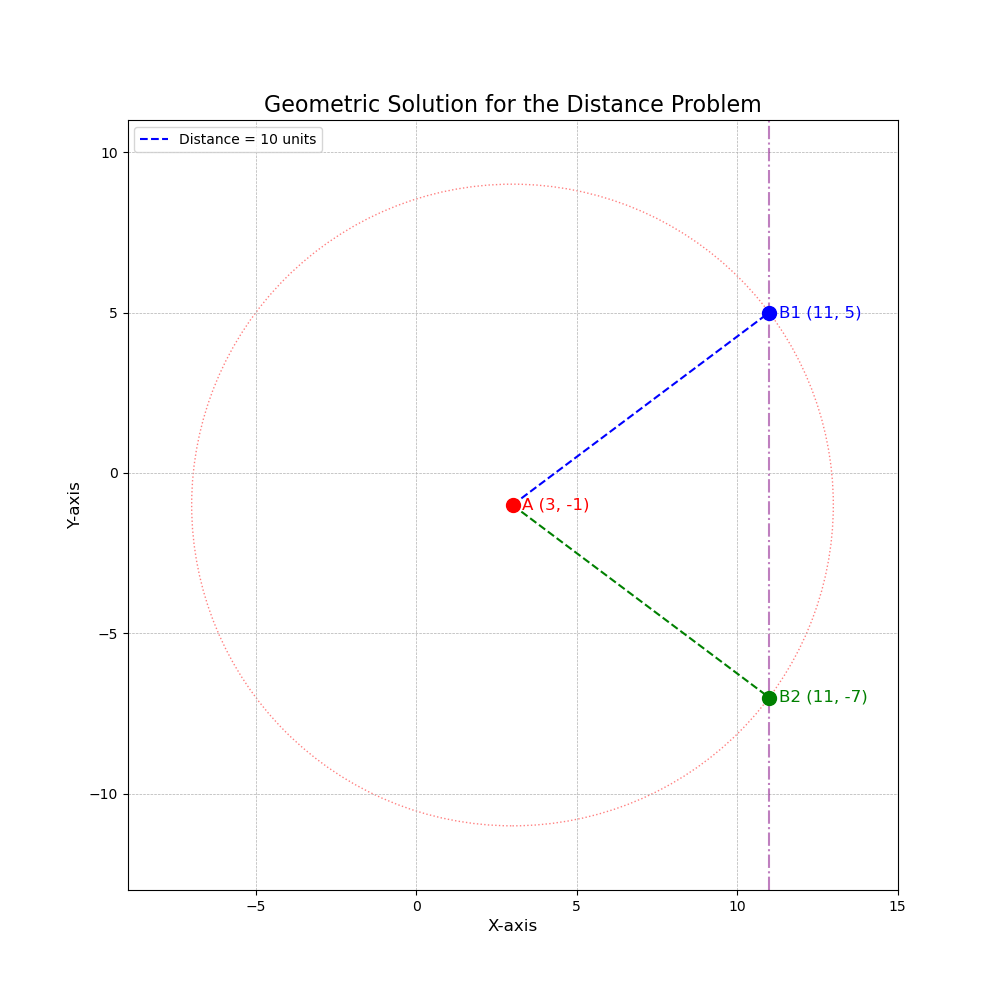
\includegraphics[width=\columnwidth]{figs/distance_plot.png}
\end{figure}
\end{document}
